\documentclass[a4paper,conference]{IEEEtran}
\usepackage{amsmath,amssymb,graphicx,booktabs,url}
\usepackage[hidelinks]{hyperref}
\title{Advertising Video Popularity Prediction:\\Auditing Creative Subgraphs and Brand Connectivity}
\author{\IEEEauthorblockN{Group 6}\IEEEauthorblockA{STAT6207: Applied Deep Learning\\The Chinese University of Hong Kong}}
\begin{document}\maketitle
\begin{abstract}
We implement a compact graph neural network (GNN) to predict cumulative YouTube views from advertising annotations. A frozen collection supplies 214 exact labels across 14 brands. The primary design is a video-level concept/evidence subgraph; video-as-node graphs are an extension. After manually merging bilingual Prudential anniversary variants, all models are retrained and evaluated on a shared campaign-grouped 80/20 split. The training-selected primary subgraph obtains log RMSE 2.402, compared with 2.375 for metadata Ridge and 2.344 for the video-node model: it does not outperform these controls. All 1,558 video-node structural pairs form complete same-brand cliques. Brand-mean and no-brand-edge controls therefore separate brand connectivity from creative-graph claims. A local Streamlit tool exposes source graphs, errors and exploratory recommendations. Cumulative snapshot labels do not validate 30-day forecasts or causal creative uplift.
\end{abstract}
\begin{IEEEkeywords}Graph neural networks, advertising, cumulative views, grouped evaluation, brand confounding.\end{IEEEkeywords}

\section{Objective, Inventory and Labels}
We predict observable video response and ask whether graph structure adds signal beyond simpler features. The target is $y_i=\ln(1+v_i)$ for cumulative views $v_i$ at collection. Neither sales nor brand recognition is measured. The supplied slide-level compact GNN is our implementation baseline: no executable VideoGNN code, weights or identifiable 120-video reference subset was provided. We use the latest full packages uniformly, without claiming an exact reproduction of that reference.

The latest version per brand gives 219 unique URLs across 14 brands; HSBC and Hang Seng use v0.2, while MTR actually contains 14 rows. Original responses are mainly in \texttt{evidence\_nodes.csv}, selecting \texttt{kind=engagement\_stats} and parsing \texttt{value\_json} or \texttt{text}. Original coverage is 219 views, 184 likes and no non-null comments; McDonald's also has direct response columns.

To collect platform labels, one unauthenticated pass over all supplied watch URLs on 9 November 2026, 12:01:03--12:02:18 UTC, recovers 214 exact current-video view counts/channel identities and 175 exact likes. No exact comments appear in initial public metadata; missing is not zero. Five URLs lacking fresh exact views are excluded, without substituting archived labels. There is no external holdout. Each retrieval retains URL/ID, UTC time, status, response digest, extraction paths and raw evidence snippets. Rounded subscriber strings are descriptive metadata, excluded from model inputs. No login barrier is bypassed.

Publication dates/durations remain source-supplied because the fresh pass exposes no verified upload dates. Exposure age is capture time minus supplied date. For the corrected training set, ages range from 36.5 to 5620.5 days (median 718.5). These are cumulative snapshot labels at heterogeneous ages, not measurements at a common horizon. A 30-day input is outside training support and cannot be called a validated 30-day prediction. Even an in-range age does not establish a validated response trajectory for a new brief.

\section{Graphs, Features and Controls}
\subsection{Primary Video Subgraph}
Each video is a graph with a context root, creative-aspect nodes and textual-evidence nodes. We normalize schema aliases, allowlist creative fields, deduplicate text, and cap repeated visual/audience aspects at four and each selected evidence kind at three. Engagement statistics, assessment/risk scores and response-bearing sentences are excluded. Across 214 graphs, 6,684 nodes and 7,780 supplied directed relations survive filtering.

Core relations are copied from \texttt{candidate\_edges.csv}: video--aspect membership, video--evidence membership, and aspect--evidence support. Original edge IDs and packages remain in the provenance table. Membership is deterministic; support links can be source-derived heuristics and are flagged. The GNN symmetrizes these edges. Figure~\ref{fig:graph} shows a real induced display subset, with no invented nodes or links; the full graph is available interactively.

\begin{figure}[t]\centering
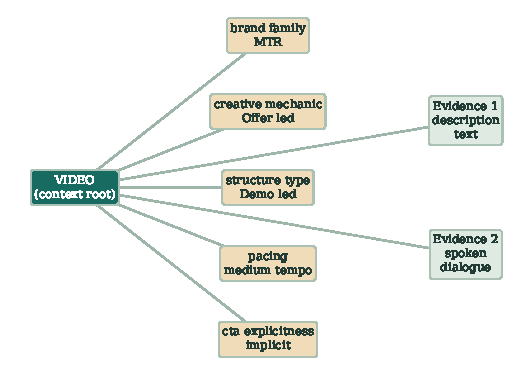
\includegraphics[width=\columnwidth]{concept_graph.pdf}
\caption{Actual training-video concept graph: source ID \texttt{cmu3gznxt000pbn5k4mu9yl5f}. An induced subset of 8 of 32 nodes is shown for legibility. Boxes show source concept values and evidence kinds; lines are original supplied membership edges. Full text, original IDs and edge provenance are exported in \texttt{report\_graph.json}.}\label{fig:graph}
\end{figure}

The root contains brand/seven creative categories, log-duration/age with missingness flags, and a 16-dimensional TF-IDF/SVD representation of message, hook, promise and CTA. Each node adds type/field indicators and a separate 16-dimensional text representation. Encoders, medians, scaling, vocabularies and SVD are fitted only on the relevant training fold. Unseen categories are handled without fitting on queries. Word tokenization limits bilingual semantic fidelity.

The tested semantic extension adds within-video edges between nonroot nodes with training-fitted SVD cosine similarity at least 0.55, up to two neighbors per node, then symmetrizes/deduplicates. This heuristic rule, node caps and input allowlists are fixed; views never construct edges. Structural-only and structural+similarity models use identical inputs and evaluation.

\subsection{Compact GNN and Feature Baselines}
Two 24-unit mean GraphSAGE layers \cite{sage,pyg} compute
\begin{equation}
 h_u^{(\ell+1)}=\operatorname{ReLU}\!\left(W_s h_u^{(\ell)}+W_n\operatorname{mean}_{w\in N(u)}h_w^{(\ell)}+b\right).
\end{equation}
A linear head on concatenated root and mean node embeddings predicts standardized log views. Adam uses learning rate 0.01 and mean squared error (MSE). A no-message MLP uses the same node information, two 24-unit transformations and root/mean readout; its parameter count differs because the GNN has neighbor weights. Additional baselines are constant training-log-mean, metadata Ridge (brand/duration/age), and Ridge on pooled raw root/mean node features.

The added brand baseline predicts the \emph{mean log views within each training brand}, using the global training log mean for unseen brands. It never averages test labels. This is a closed-form MSE fit, not an arithmetic mean of raw views. All baselines share the target, split and quantitative metrics.

\subsection{Video Nodes: Brand Connectivity Audit}
The extension represents each video as a node, using root features and two mean GraphSAGE layers. Supplied same-brand/author/creative-category relations are collapsed to binary adjacency. Crucially, the resulting 1,558 unique pairs equal complete brand cliques: every edge joins same-brand videos. Overlapping creative/author labels add no distinct adjacency. Thus a good result cannot demonstrate that creative-concept relationships are effective.

The no-brand-edge control removes \emph{every same-brand endpoint pair}, including overlaps supported by other relation labels. Zero edges remain. It retains brand input features, architecture and the same tuning grid, so this is an adjacency ablation, not removal of all brand information. The separate similarity extension adds five nearest training-feature neighbors. Query nodes receive messages only from training references; they send none to training or other query nodes.

\section{Training and Corrected Evaluation}
\subsection{Campaign-Grouped 80/20 Split}
Original groups union normalized same-brand campaign labels and exact same-brand message duplicates. Manual review identified Prudential 170th-anniversary variants \texttt{jlB5oiVibQU} and \texttt{m8qVqW63VQs}, previously separated by English/Chinese naming and split across train/test. Both are now assigned the canonical ID \texttt{prudential\_170th\_anniversary\_2019}; a checked-in override table unions their existing groups rather than splitting any prior family.

There are now 198 groups. We resplit all models into 171 training and 43 testing videos (79.91/20.09\%). The pre-existing count-only rule takes the first seed from 42 yielding exactly round$(0.2N)$ query videos; this gives seed 50. It uses group sizes, never view labels or model scores. Both anniversary variants are now in training; outer and inner-fold group/URL disjointness are checked. Other paraphrased families may still escape this heuristic-plus-manual grouping. This measures unseen campaign groups within known brands, not unseen-brand transfer.

This is explicitly a \emph{post-audit corrected internal evaluation}. Earlier holdout errors were inspected before the grouping correction; the new split is not a pristine external test. Superseded metrics and the reason for correction are preserved. The frozen label snapshot is unchanged.

\subsection{Quantitative Objectives and Selection}
Three grouped folds inside the outer training set select Ridge $\alpha\in\{10,100\}$ and neural weight decay $\lambda\in\{0.01,0.1\}$. Each fold refits all preprocessing. Early stopping uses fold-validation log MSE, at most 260 epochs and patience 35. Hyperparameters minimize mean fold log RMSE; final fitting uses all 171 training videos and the median selected-fold stopping epoch, without querying test losses. Closed-form mean baselines have no tuning parameters.

The primary graph design remains subgraph-as-video. Within that prespecified family, training CV now selects \emph{structural-only}, with 24 epochs and $\lambda=0.1$. Its training log RMSE is 2.088. Across the comparison suite, training CV selects the no-brand-edge video-node control; we disclose this without redefining the primary design or choosing a new primary model from test rankings. Objectives, fold scores, final training RMSE/loss histories, configurations and source hashes are exported for every model.

Common held-out metrics are MAE/RMSE on natural-log views and Spearman correlation. The inverse $\exp(\hat y)-1$ is clipped to nonnegative counts; it is not an unbiased arithmetic expected view count. A 2,000-draw campaign-level bootstrap gives conditional intervals and paired differences, excluding split/selection uncertainty. Additional seeds 7, 21 and 84 probe initialization without replacing seed 42.

\begin{table}[t]\caption{Corrected same-split test results ($n=43$). Lower errors are better. Bold marks the training-selected primary subgraph, not the best test result.}\label{tab:main}\centering\footnotesize\setlength{\tabcolsep}{3pt}
\begin{tabular}{lrrr}\toprule
Model & Log MAE & Log RMSE & $\rho$\\\midrule
Constant log mean & 2.282 & 2.646 & -- \\
Training brand log mean & 1.989 & 2.622 & 0.281 \\
Metadata Ridge & 1.989 & 2.375 & 0.408 \\
Pooled-feature Ridge & 1.904 & 2.345 & 0.450 \\
No-message MLP & 1.827 & 2.360 & 0.436 \\
\bfseries Subgraph: structural & 1.795 & 2.402 & 0.447 \\
Subgraph: structural+sim. & 1.917 & 2.286 & 0.490 \\
Video node: brand cliques & 1.952 & 2.344 & 0.550 \\
Video node: cliques+sim. & 1.886 & 2.369 & 0.414 \\
Video node: no brand edges & 1.948 & 2.382 & 0.362 \\
\bottomrule\end{tabular}\end{table}

\section{Results and Failure Analysis}
The original, superseded primary result (RMSE 2.238) was worse than metadata Ridge (2.134) and video-node GNN (2.099); it did not justify a superiority claim. After correcting grouping and retraining, the primary structural subgraph obtains RMSE 2.402 (95\% campaign-bootstrap interval [1.759, 2.939]), again worse than metadata Ridge (2.375), pooled Ridge (2.345) and video-node brand cliques (2.344). Its paired RMSE difference versus metadata Ridge has interval [-0.222, 0.249], spanning zero. We establish neither superiority nor a precise performance ordering.

The similarity subgraph has test RMSE 2.286, but structural-only was preferred by training CV; we do not switch models after seeing testing results. In particular, the primary MAE/RMSE tradeoff and uncertain edge gains do not prove useful creative graph structure beyond feature baselines.

Brand mean gives RMSE 2.622; video-node brand cliques give 2.344, versus 2.382 with no edges. The paired clique-minus-no-edge RMSE interval [-0.215, 0.142] includes zero. Thus adjacency supplies only a small, uncertain numerical gain here. The clique model also uses duration, age and creative root features, so improvement over brand mean cannot be attributed solely to edges or concepts.

\begin{figure}[t]\centering
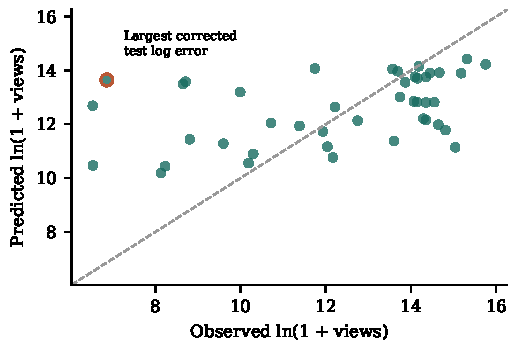
\includegraphics[width=\columnwidth]{scatter.pdf}
\caption{All 43 corrected test predictions from the primary structural subgraph. Dashed line: perfect log-scale prediction. The circled IKEA case is the largest corrected test log error; extreme responses are compressed.}\label{fig:scatter}
\end{figure}

\subsection{Reupload and Exposure Confounding}
A particularly informative \emph{historical} failure is the 1996 McDonald's ad reupload \texttt{P25f\_dDd2MI}: observed views were 1,019, while the superseded subgraph predicted about 442,536. The captured uploader is ``TPB HK CM,'' a third-party Hong Kong TV-ad archive, rather than the official brand channel. Its supplied upload date is 28 April 2026 (about 195.5 days before capture); 1996 refers to the creative, not the upload age. Brand/creative cues do not establish comparable distribution or paid exposure. This is a plausible channel/exposure mismatch, not an identified causal explanation.

That video is now in training, so its corrected prediction is an in-sample diagnostic, \emph{not} a held-out error. The corrected largest test log error instead concerns IKEA video \texttt{4rixed7cNhI}: 958 observed versus 839,933 predicted views. An official uploader alone therefore does not resolve exposure confounding. Figure~\ref{fig:scatter} and exported view-scale/brand slices make the remaining failures visible.

\subsection{Cross-Brand Stress Test}
Leave-one-brand-out (LOBO) refits on 13 brands and tests the remaining brand, repeating all 14. An inner grouped holdout chooses epochs; regularization is fixed separately ($\alpha=100$, $\lambda=0.1$), never tuned using held-out-brand responses. Brand mean necessarily falls back to the global training log mean. Table~\ref{tab:lobo} reports macro averages; constant-within-brand predictions have undefined rank correlation. These 70 model--brand runs are a stress test separate from the main split, with small per-brand samples and substantial transfer error.

\begin{table}[t]\caption{LOBO brand-macro results across 14 held-out brands.}\label{tab:lobo}\centering\footnotesize\setlength{\tabcolsep}{3pt}
\begin{tabular}{lrrr}\toprule
Model & Log MAE & Log RMSE & $\rho$\\\midrule
Pooled-feature Ridge & 2.145 & 2.563 & 0.262 \\
No-message MLP & 2.188 & 2.634 & 0.237 \\
Subgraph: structural & 2.134 & 2.593 & 0.212 \\
Subgraph: structural+sim. & 2.136 & 2.589 & 0.174 \\
Training brand log mean & 2.261 & 2.672 & -- \\
\bottomrule\end{tabular}\end{table}

\section{Recommendations, Website and Limitations}
Six cases use the first six corrected test indices, without selecting maximum gains. Each follows objective $\rightarrow$ creative elements $\rightarrow$ predicted/observed response with uncertainty $\rightarrow$ transferable hypothesis. The frozen primary GNN searches mechanic/structure/pacing triples appearing at least twice in training, with at most two categorical edits. Original settings remain if no candidate improves the model estimate; text/similarity features are recomputed. Existing source evidence stays fixed, so a suggested category can conflict with the script and requires human revision.

For the HSBC case \texttt{cmsxzrhfa0017bnn8p2stilmd}, observed views are 1,709,054; predictions are 189,946 before and 975,602 after the suggested settings. Linked supporting examples come only from training. Out-of-fold absolute-log-residual sensitivity bands are reported; these are not calibrated individual intervals, and no modified-video response is observed.

The 30-second new-brief storyboard uses training-median age 718.5 days, \emph{not} a 30-day forecast. It contains a hook (0--3 s), product benefit (3--20 s), suggested structure (20--27 s), and CTA (27--30 s). A graph built solely from declared inputs avoids borrowing another video's evidence, but is sparser than extracted training graphs. New briefs remain an unvalidated showcase even at in-range ages.

The local Streamlit/Python website directly loads the frozen PyG checkpoint and encoders. It combines editable feature-to-recommendation inputs, source evidence, actual concept graphs, baseline/ablation results and one storyboard. Display-edge toggles do not change the trained model. New inputs default to the training age median; out-of-range inputs, including 30 days, display an explicit extrapolation warning in the page and prediction JSON. All outputs remain exploratory cumulative-view estimates. Numerical checks cover all 214 frozen predictions and six optimizations; widget tests cover both input types, graph controls and age warnings.

Paid spend, targeting, channel audience, publication timing, reupload status and featured people's popularity can jointly affect both creative choices and views. Contemporary channel metadata is not historical audience exposure. Annotation style, heuristic support edges, bilingual tokenization, incomplete responses, imperfect campaign verification and a single corrected split further constrain construct validity. Optimizing model estimates can exploit prediction errors; support from two examples does not identify causal uplift.

Priority improvements are to verify campaign families, uploader type and dates; collect exposure/spend and fixed-age response labels; expand a separately frozen official-channel holdout; test bilingual encoders and capacity-matched edge controls; and repeat grouped/time splits. Prospective exposure-controlled coherent variants are required to evaluate actual creative gains. We claim no sales, brand-recognition or causal engagement effect.

\section{Conclusion}
The corrected compact-GNN baseline is reproducible and quantitatively evaluated, but the primary concept subgraph does not outperform simpler controls. Video-node adjacency is exactly brand connectivity, and its no-edge comparison is uncertain. Cumulative snapshot prediction must be separated from validated future-horizon forecasting. The contribution is an auditable comparison and source-linked hypothesis tool, rather than proof that concept edges improve creative performance. This report uses the IEEE A4 template \cite{ieee}; code, frozen evidence, checkpoints, full metrics and session transcript accompany it.

\begin{thebibliography}{3}
\bibitem{sage} W. L. Hamilton, R. Ying, and J. Leskovec, ``Inductive representation learning on large graphs,'' in \emph{Advances in Neural Information Processing Systems}, vol. 30, 2017.
\bibitem{pyg} PyTorch Geometric, ``SAGEConv and graph-level pooling documentation.'' [Online]. Available: \url{https://pytorch-geometric.readthedocs.io/}
\bibitem{ieee} IEEE, ``Manuscript templates for conference proceedings.'' [Online]. Available: \url{https://www.ieee.org/conferences/publishing/templates.html}
\end{thebibliography}\end{document}
